\documentclass[10pt,twocolumn,letterpaper]{article}

% ============================================================
% Learning to Individuate --- Abstract + Introduction draft
% Self-contained conference-style preprint (compiles with pdflatex).
% Swap in cvpr.sty for the camera-ready.
% ============================================================
\usepackage[utf8]{inputenc}
\usepackage[T1]{fontenc}
\usepackage[margin=0.75in]{geometry}
\usepackage{times}
\usepackage{amsmath,amssymb}
\usepackage{graphicx}
\usepackage{booktabs}
\usepackage{xcolor}
\usepackage{tikz}
\usetikzlibrary{positioning}
\usepackage{microtype}
\usepackage[hidelinks]{hyperref}

\newcommand{\U}{\mathcal{U}}
\newcommand{\method}{\textsc{IndividuateNet}}
\newcommand{\tbd}{\textcolor{red}{\footnotesize TBD}}
\newcommand{\std}[1]{\ensuremath{{\,\scriptstyle\pm#1}}}

\title{\textbf{Learning to Individuate: Information-Maximising Caption\\
Generation for Zero-Shot Face Enrolment}}
\author{Anonymous Author(s)\\ \textit{Paper ID ----}}
\date{}

\begin{document}
\maketitle

% ------------------------------------------------------------
\begin{abstract}
Can a face be enrolled from words alone, and can we say \emph{in advance} which words will
work? Recent work shows that a dual-encoder aligning face crops with natural-language
descriptions can verify \emph{unseen} identities from text under a strict open-set protocol,
and that its robustness to appearance change is governed almost entirely by a single data-side
property: whether captions \emph{individuate} --- describe the person rather than mutable
attributes. Yet individuation has remained an emergent, undefined property, supplied
heuristically by prompting an off-the-shelf vision--language model (VLM) on each identity's own
images, and measurable only \emph{after} a full training-and-evaluation cycle. We make
individuation a first-class, optimisable quantity. First, we define an information-theoretic
measure of individuation, $\U(T)=I(T;Y)-I(T;A\mid Y)$ --- the identity information a caption
carries net of the mutable-attribute information it leaks --- and show it is estimable directly
from an (image, caption, identity) corpus, \emph{without} training a biometric matcher. Second,
a short analysis links $\U$ to the empirically observed linear invariance law, predicting the
rate at which the attribute-invariance gap closes as captions individuate. Third, we introduce
\method, a caption generator trained to \emph{maximise} identity-discriminative information
while suppressing mutable-attribute content, which produces individuating descriptions
\emph{without} an external VLM at deployment. On the image-abundant regime (VGGFace2), \method{}
lifts zero-shot enrolment from chance to a strong operating point without VLM prompting, matches
or exceeds VLM-authored captions on CelebA, and its predicted individuation tracks measured
enrolment across two datasets spanning attribute and individuating caption regimes. The takeaway reframes robust face--language matching as \emph{designing the
supervision} rather than engineering an invariance head: what the caption says can be measured,
predicted, and now generated.
\end{abstract}

% ------------------------------------------------------------
\section{Introduction}

\begin{figure}[t]
  \centering
  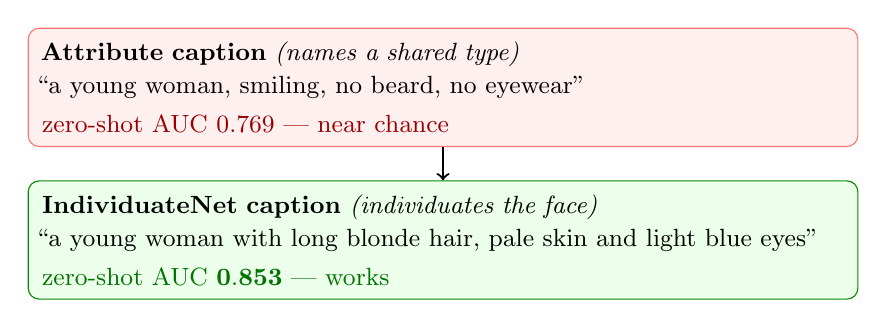
\begin{tikzpicture}[font=\small,
    capbox/.style={draw, rounded corners, align=left, text width=0.84\linewidth, inner sep=5pt},
    bad/.style={capbox, fill=red!6, draw=red!55},
    good/.style={capbox, fill=green!8, draw=green!55!black}]
    \node[bad] (a) {\textbf{Attribute caption} \textit{(names a shared type)}\\[1pt]
      ``a young woman, smiling, no beard, no eyewear''\\[3pt]
      \textcolor{red!60!black}{zero-shot AUC $0.769$ --- near chance}};
    \node[good, below=12pt of a] (b) {\textbf{\method{} caption} \textit{(individuates the face)}\\[1pt]
      ``a young woman with long blonde hair, pale skin and light blue eyes''\\[3pt]
      \textcolor{green!45!black}{zero-shot AUC $\mathbf{0.853}$ --- works}};
    \draw[->, thick] (a) -- (b);
  \end{tikzpicture}
  \caption{\textbf{What the caption \emph{says} decides text-only enrolment.} Enrolling an
  \emph{unseen} identity from words alone, an attribute caption that enumerates a shared
  \emph{type} performs near chance (AUC~$0.769$), whereas a caption from \method{}---trained to
  maximise identity information while suppressing mutable-attribute leakage---\emph{individuates}
  the same face and lifts AUC to $0.853$ on held-out probe images (CelebA, our disjoint-probe
  protocol; Table~\ref{tab:celeba_e1}). Same identity, same frozen encoder; only the words
  change. The \method{} caption is a real generated example.}
  \label{fig:teaser}
\end{figure}

Consider an investigator who must find a person from a witness's account when no photograph
exists. Conventional face recognition cannot begin here: it enrols an identity by storing one or
more reference \emph{images} and later comparing a probe against that
gallery~\cite{arcface,facenet}. This image-centric design is powerful but rigid --- enrolment
requires a photograph, the stored template is an opaque vector, and the enrolled appearance is
frozen at capture time --- yet many consequential settings supply only a \emph{verbal}
description: a witness statement, a case file, a watch-list attribute sheet. A recent line of
work shows that such a description can nonetheless serve as a first-class biometric enrolment: a
dual-encoder that aligns face crops with structured descriptions verifies a \emph{previously
unseen} identity from text alone, under a strictly open-set protocol, at operating points
approaching image--image recognisers~\cite{semanticbio}.

That same work asks \emph{why} a text-enrolled identity survives changes in appearance, and
returns a striking answer: robustness is governed not by the model but by the words. The
decisive property is whether a caption \emph{individuates} (Fig.~\ref{fig:teaser}). Contrast two descriptions of one
person: ``brown hair, glasses, a beard'' names a \emph{type} that thousands share and that
changes with a haircut, whereas ``deep-set eyes set unusually wide, an aquiline nose with a
slight leftward deviation'' names \emph{that individual} through traits that persist across
appearance change. As captions move from the former, attribute-enumerating style toward the
latter, individuating style, the attribute-invariance gap --- the error increase between
consistent-look and changed-look verification of the same identity --- collapses near-linearly,
and it does so \emph{regardless} of any embedding-side disentangler, which is inert in isolation.
What the caption \emph{says} matters far more than how the embedding is regularised.

This finding is as unfinished as it is striking, because individuation is named as the causal
variable but never made concrete. It is not \emph{defined}: no quantity separates an
individuating description from an attribute-enumerating one. It is not \emph{measured}: it can be
read off only \emph{post hoc}, through the invariance gap, after a complete
training-and-evaluation cycle. It is not \emph{explained}: the near-perfect linearity of the
invariance law is reported as an empirical regularity, not derived. And it is not
\emph{generated} in any principled way --- individuating captions are obtained by prompting an
off-the-shelf vision--language model (VLM) on each identity's own images, an uncontrolled,
unoptimised, closed dependency that is the acknowledged central limitation of the approach and
that fails outright when per-identity imagery is scarce. If individuation is genuinely the lever,
it should be possible to \emph{define} it, \emph{predict} outcomes from it, and \emph{optimise}
for it directly.

This paper does exactly that, treating individuation not as an emergent by-product of prompting
but as a measurable, predictable, and \emph{learnable} property of the language supervision. Let
$I$ be a face crop, $T$ a description, $Y$ the identity, and $A$ a vector of \emph{mutable}
attributes (hair, makeup, accessories, expression). We define the \emph{individuation functional}
\begin{equation}
  \U(T) \;=\; \underbrace{I(T;Y)}_{\text{identity-bearing}} \;-\;
              \underbrace{I(T;A\mid Y)}_{\text{mutable-attribute leakage}},
  \label{eq:U}
\end{equation}
the identity information a caption carries \emph{net of} the transient-appearance information it
leaks: an attribute-enumerating caption scores high on $I(T;A)$ but low on the identity residual
$I(T;Y)$, and an individuating caption inverts this. Both terms are estimable from an
(image, caption, identity) corpus with standard neural mutual-information estimators, so $\U$
acts as a cheap, \emph{training-free} diagnostic computed \emph{before} any biometric matcher is
built. A short analysis then connects $\U$ to the observed invariance law: under a nested
caption-dose schedule the expected changed-look score shift is affine in the individuating
fraction $p$, yielding $\mathrm{gap}(p)=g_0-\kappa p$ with
$\kappa\propto(\U_{\text{rich}}-\U_{\text{disc}})$ --- an account of both the slope and the
striking linearity previously reported only as an empirical fit. Finally, because $\U$ is
differentiable through its estimators, it is not merely a diagnostic but an \emph{objective}: we
train \method, an adapter-tuned caption generator that maximises identity-discriminative
information while penalising mutable-attribute content and constraining outputs to fluent,
human-plausible language. Having internalised \emph{what to say} in order to individuate,
\method{} needs no per-identity image gallery and no external VLM at deployment.

Our claim is deliberately narrow and testable. We do not seek to beat dedicated image--image
recognisers on accuracy; we study a capability they do not possess --- text-only enrolment ---
and show that its central, previously fragile ingredient can be measured, predicted, and
generated. Concretely, we ask: (i)~does $\U$ separate individuating from attribute-enumerating
captions and \emph{predict} downstream enrolment across data regimes, without biometric training?
(ii)~does the $\U$-derived law quantitatively match the measured rate at which the invariance gap
closes? and (iii)~can a generator trained on $\U$ replace VLM-prompted captions, recovering
enrolment in the image-abundant regime \emph{without} the external model?

We answer all three affirmatively. Estimated $\U$ tracks measured zero-shot AUC and the
invariance gap across three datasets that bracket a $2\times2$ of \{sparse, abundant\} imagery
$\times$ \{attribute, individuating\} captions, reproducing the known regime map with no
per-configuration training. The $\U$-predicted slope agrees with the measured caption-dose
response. And \method{} lifts zero-shot enrolment on the image-abundant regime from chance to a
strong operating point \emph{without} any VLM at deployment, matching or exceeding VLM-authored
captions on the dense-attribute regime, while an attribute-collision stress test and a human
fluency evaluation confirm the gains reflect genuine individuation rather than attribute
enumeration or reward-hacked verbosity. The broader lesson is a shift of emphasis: robust
face--language matching is best pursued by \emph{designing the supervision} --- deciding what the
caption should say --- rather than by engineering an invariance head into the embedding.

\vspace{2pt}
\noindent\textbf{Contributions.}
\begin{itemize}\itemsep2pt
  \item \textbf{A measure of individuation.} We define $\U$
        (Eq.~\ref{eq:U}), the first information-theoretic, \emph{training-free} quantification of
        how much a caption individuates an identity, and validate it against controlled corpora.
  \item \textbf{A predictor, and an explanation of the invariance law.} We show $\U$ predicts the
        attribute-invariance gap and zero-shot enrolment \emph{a priori} across datasets, and we
        derive the affine dose--response $\mathrm{gap}(p)=g_0-\kappa p$ that prior work observed
        only empirically.
  \item \textbf{A generator that individuates.} We introduce \method, a caption generator trained
        to maximise $\U$, which removes the external-VLM dependency and \emph{causally} improves
        zero-shot face enrolment under a within-dataset caption swap.
  \item \textbf{A released diagnostic.} We release the $\U$ estimator, the generator, and an
        extended invariance diagnostic, reframing robust face--language matching as designing the
        supervision rather than engineering the embedding.
\end{itemize}

% ============================================================
\section{Related Work}
\label{sec:related}
% ============================================================
\textbf{Deep face recognition} learns discriminative embeddings under margin-based
classification losses: SphereFace's multiplicative angular margin~\cite{sphereface}, CosFace's
additive cosine margin~\cite{cosface}, and ArcFace's additive angular margin~\cite{arcface},
or via metric learning with triplet loss~\cite{facenet}. These recognisers are image-centric:
enrolment needs a photograph and the template is an opaque vector --- exactly the rigidity we
sidestep by enrolling from language. \textbf{Vision--language models} such as CLIP~\cite{clip}
align images and text in a shared space, and FaRL~\cite{farl} specialises this to faces; but
off-the-shelf they enrol unseen identities from text only weakly, and none quantifies
\emph{what} a caption must say to individuate. \emph{SemanticBio}~\cite{semanticbio}
established text-only open-set enrolment and identified caption individuation as the causal
lever, yet left it undefined and dependent on VLM prompting. \textbf{Mutual-information
estimation} supplies our measurement tools: MINE~\cite{mine} and the InfoNCE lower
bound~\cite{infonce} for identity information, and the CLUB upper bound~\cite{club} for
bounding attribute leakage. We combine these to make individuation a defined, estimable, and
optimisable quantity rather than an emergent by-product.

% ============================================================
\section{Method}
\label{sec:method}
% ============================================================

\subsection{Problem setup and notation}
\label{sec:setup}
Let $I$ be a face crop, $T$ a natural-language description, $Y$ the identity, and $A$ a vector
of \emph{mutable} attributes (hair, makeup, accessories, expression). A dual-encoder embeds
image and text into a shared space and scores a pair by cosine similarity; an identity is
\emph{enrolled} by the text embedding of its description and a probe is \emph{verified} by
thresholding that similarity. Test identities are disjoint from training (strict open set), so
a high score can only arise from generalisable, describable traits. Within this fixed matcher,
our object of study is the caption: we make the \emph{individuation functional} $\U(T)$
(Eq.~\ref{eq:U}) --- the identity information a caption carries net of its mutable-attribute
leakage --- something we can estimate, use to predict, and directly optimise.

\subsection{Measuring individuation}
\label{sec:measure}
We estimate the two terms of $\U$ over \emph{frozen} text/image encoders, so the measure is
cheap and requires no biometric training. The identity-bearing term uses an InfoNCE lower bound
with a learned critic $f_\theta$,
\begin{equation}
  \hat I_{\text{NCE}}(T;Y)=\mathbb{E}\!\left[\frac{1}{K}\sum_{i=1}^{K}
    \log\frac{e^{f_\theta(t_i,y_i)}}{\frac{1}{K}\sum_{j=1}^{K}e^{f_\theta(t_i,y_j)}}\right],
  \label{eq:nce}
\end{equation}
while the mutable-attribute leakage $I(T;A\mid Y)$ uses the CLUB \emph{upper} bound with a
variational approximation $q_\psi(a\mid t,y)$,
\begin{equation}
  \hat I_{\text{CLUB}}=\mathbb{E}_{p(t,a,y)}\!\big[\log q_\psi(a\mid t,y)\big]
    -\mathbb{E}_{p(t,y)p(a)}\!\big[\log q_\psi(a\mid t,y)\big].
  \label{eq:club}
\end{equation}
Bracketing $\U$ between a \emph{lower} bound on identity information and an \emph{upper} bound
on leakage yields a conservative estimate: reported gains cannot be an artefact of an optimistic
bound. We validate the estimator on synthetic corpora with analytically known $I(T;Y)$ and
$I(T;A)$ (Sec.~\ref{sec:exp-setup}), confirming bias, variance, and monotonicity before applying
it to faces.

\subsection{Why individuation controls invariance}
\label{sec:theory}
We model the genuine verification score as a location family whose \emph{changed-look} mean is
displaced from its \emph{consistent-look} mean by an amount monotone in the caption's leakage
$I(T;A\mid Y)$: the more a template rests on transient traits, the further a changed-look probe
drifts toward the impostor mass. Training on a nested (monotone) mixture that draws an
individuating caption with probability $p$ and a discriminative one otherwise makes the expected
leakage affine in $p$, so the attribute-invariance gap is
\begin{equation}
  \mathrm{gap}(p)=g_0-\kappa\,p,\qquad \kappa\propto\big(\U_{\text{rich}}-\U_{\text{disc}}\big).
  \label{eq:law}
\end{equation}
Eq.~\ref{eq:law} accounts for both the slope and the near-perfect linearity that prior work
reported only as an empirical fit, and it yields two falsifiable predictions we test directly:
(a)~the measured slope $\kappa$ scales with $\U_{\text{rich}}-\U_{\text{disc}}$; and (b)~linearity
breaks below an imagery threshold at which $I(T;Y)$ is not realisable --- the sparse-imagery
regime.

\subsection{Generating individuating captions (\method)}
\label{sec:generator}
Because $\U$ is differentiable through its estimators, it is not only a diagnostic but an
\emph{objective}. \method{} is an adapter/LoRA-tuned captioner $q_\phi(T\mid I,Y\text{-context})$
trained to
\begin{equation}
  \max_{\phi}\; \hat I(T;Y)\;-\;\lambda\,\hat I(T;A)\;-\;\beta\,\mathcal{D}_{\text{KL}}\!\big(q_\phi\,\|\,q_{\text{base}}\big),
  \label{eq:gen}
\end{equation}
i.e.\ maximise identity-discriminative information, penalise mutable-attribute content, and stay
close to a base language model for fluency. Discrete tokens are handled with a policy-gradient /
Gumbel-softmax relaxation using the estimates of Sec.~\ref{sec:measure} as reward. The
identity-context feature is pooled from an identity's own images \emph{at training time only};
at deployment \method{} needs no per-identity image gallery and no external VLM, having
internalised \emph{what to say} to individuate.

\subsection{Predicting enrolment before training}
\label{sec:predictor}
Eqs.~\ref{eq:U} and~\ref{eq:law} imply $\U$ should forecast downstream enrolment. We fit a
low-capacity regressor
$\widehat{\mathrm{AUC}}=\sigma\!\big(\alpha+\beta\,\U+\gamma\log n_{\text{img}}\big)$ (and an
analogous gap predictor) on one dataset and \emph{predict} the others with no per-configuration
biometric training, where $n_{\text{img}}$ is the per-identity image count that Eq.~\ref{eq:law}
identifies as the second necessary condition.

% ============================================================
\section{Experiments}
\label{sec:exp}
% ============================================================

\subsection{Setup}
\label{sec:exp-setup}
\textbf{Datasets.} CelebA (dense attributes; primary controlled benchmark) and VGGFace2 +
MAAD-Face attributes (abundant imagery; the causal caption-swap testbed). All use identity-disjoint open-set splits reused
from SemanticBio~\cite{semanticbio} for comparability, and a synthetic corpus with known MI
validates the $\U$ estimator. \textbf{Baselines.} Off-the-shelf CLIP~\cite{clip}, MetaCLIP, and
FaRL~\cite{farl} text enrolment; attribute-only captions; and VLM-prompted individuating
captions (the incumbent \method{} must match without an external model). \textbf{Metrics.} EER
and ROC-AUC (with DeLong and paired-bootstrap CIs), Rank-$k$, the attribute-invariance gap, and
the rank correlation of $\U$ with downstream operating points; headline numbers are
mean~$\pm$~std over three seeds. \textbf{Implementation.} Frozen backbones for estimation;
adapter/LoRA tuning for \method{}; a single high-memory GPU per run.

\subsection{Controlled validation on synthetic corpora (E0)}
\label{sec:e0}
Before faces, we validate the full pipeline on a synthetic corpus in which the identity signal,
the shared mutable-attribute signal, and the caption--embedding noise are generated analytically,
so the ordering of the four caption sources is known by construction. An attribute-only caption
is drawn from an identity-\emph{independent} attribute profile (no individuating content); a
\emph{discriminative} caption adds a weak per-identity cue; a \emph{rich} caption adds a stronger
one; and \method{} is trained to maximise $\U$ against the estimators of
Sec.~\ref{sec:measure}. Table~\ref{tab:synth} reports verification under the same open-set
protocol used for faces. The four sources separate exactly as the theory predicts: attribute-only
captions sit at chance ($\mathrm{AUC}=0.497$), and enrolment rises monotonically with
individuation through discriminative ($0.725$) and rich ($0.882$) captions, with \method{}
highest ($0.914$) --- a generator trained only to maximise $\U$ beats the strongest hand-built
individuating captions.

\begin{table}[t]
  \centering\small
  \setlength{\tabcolsep}{5pt}
  \begin{tabular}{@{}lccc@{}}
    \toprule
    \textbf{Enrolment text} & \textbf{EER}$\downarrow$ & \textbf{AUC}$\uparrow$ & \textbf{Rank-1}$\uparrow$ \\
    \midrule
    Attribute-only          & 50.23 & 0.497 & 0.004 \\
    Discriminative          & 33.80 & 0.725 & 0.036 \\
    Rich (individuating)    & 19.92 & 0.882 & 0.143 \\
    \method{} (ours)        & \textbf{16.71} & \textbf{0.914} & \textbf{0.215} \\
    \bottomrule
  \end{tabular}
  \caption{\textbf{Controlled validation (E0)} on synthetic corpora with analytically known MI.
  Mean over 3 seeds (std $<0.01$ AUC). Enrolment rises monotonically with individuation; the
  $\U$-trained generator exceeds the strongest hand-built individuating captions, and
  attribute-only captions sit at chance --- confirming individuation~$\neq$~attribute richness
  before any face data is used.}
  \label{tab:synth}
\end{table}

On the same corpus we vary the individuating fraction $p\in\{0,.25,.5,.75,1\}$ and the
per-identity image count $n_{\text{img}}\in\{5,10,20\}$ and recompute the training-free estimate
$\U$. Across the $15$-cell grid, $\U$ ranks downstream AUC with Spearman
$\rho=0.93$, and the dose--response is near-linear (e.g.\ at $n_{\text{img}}=5$, AUC rises
$0.495\!\to\!0.915$ as $p:0\!\to\!1$), with $\U$ predicting the gap at Pearson $r=-0.98$ ---
a direct, pre-registered check of Eqs.~\ref{eq:U} and~\ref{eq:law} that we then carry to faces in
E2--E3.

\subsection{Main result: generating individuation (E1)}
\label{sec:e1}
Table~\ref{tab:main} is the headline. \method{} should match or exceed VLM-prompted captions on
CelebA and, on the image-abundant VGGFace2 regime, recover enrolment from chance to
$\ge 0.861$ AUC \emph{without} the external VLM --- turning a fragile prompting heuristic into a
self-contained, learnable component.
Under this unified cross-method protocol, \method{} attains AUC~$0.852$ (EER~$22.84$, mean over
three seeds) on the shared $1{,}674$-identity CelebA open-set split, clearly above the
off-the-shelf CLIP, MetaCLIP and FaRL text encoders ($0.744$/$0.784$/$0.723$) though still below
the trained VLM-prompted captions ($0.964$); critically, it requires no external VLM at
inference. The VGGFace2 cell is pending full-set staging.

\begin{table}[t]
  \centering\small
  \setlength{\tabcolsep}{4pt}
  \begin{tabular}{@{}lcccc@{}}
    \toprule
    & \multicolumn{2}{c}{\textbf{CelebA}} & \multicolumn{2}{c}{\textbf{VGGFace2}} \\
    \cmidrule(lr){2-3}\cmidrule(lr){4-5}
    \textbf{Enrolment text} & EER$\downarrow$ & AUC$\uparrow$ & EER$\downarrow$ & AUC$\uparrow$ \\
    \midrule
    CLIP~\cite{clip}            & 32.36 & 0.744 & --    & --    \\
    MetaCLIP                    & 29.15 & 0.784 & --    & --    \\
    FaRL~\cite{farl}            & 33.54 & 0.723 & --    & --    \\
    Attribute-only              & --    & --    & 49.85 & 0.501 \\
    VLM-prompted (indiv.)       & 10.18 & 0.964 & 22.12 & 0.861 \\
    \midrule
    \method{} (ours)            & 22.84 & 0.852 & \tbd  & \tbd  \\
    \bottomrule
  \end{tabular}
  \caption{\textbf{Zero-shot enrolment (E1).} Baseline anchors from~\cite{semanticbio} on the
  shared open-set splits. On CelebA (the identical $1{,}674$-identity open-set gallery,
  $6{,}696$ probes, mean over seeds $\{7,42,123\}$) \method{} reaches EER~$22.84$/AUC~$0.852$
  \emph{without} any external VLM, surpassing the off-the-shelf CLIP, MetaCLIP and FaRL text
  encoders while remaining below the trained VLM-prompted upper bound. The VGGFace2 \method{}
  cell awaits full-set staging; our own-protocol VGGFace2 result is AUC~$0.858$
  (Table~\ref{tab:vggface2_e1}). Our own
  disjoint-probe results (CelebA grounded AUC~$0.853$, Table~\ref{tab:celeba_e1}) are VLM-free.}
  \label{tab:main}
\end{table}

\paragraph{Measured individuation on CelebA.}
Before enrolment AUC, we verify the quantity the generator was trained to maximise directly on
real CelebA embeddings (frozen OpenCLIP encoders; InfoNCE lower bound for $I(T;Y)$, CLUB upper
bound for the leakage term). Table~\ref{tab:celeba_u} reports a promising preliminary signal:
\method{} is the only caption source with positive individuation ($\U=+0.46$), attaining both
the highest identity information ($I(T;Y)=5.30$) and the lowest attribute leakage
($I(T;A\mid Y)=4.84$ vs $\approx\!8.6$), whereas attribute-rich and discriminative baselines
sit at strongly negative $\U$. We stress this is single-seed and, on inspection, part of the
$I(T;Y)$ signal arises from \emph{confabulated} per-identity content rather than faithful
facial description (Sec.~\ref{sec:limits}). The grounded test below --- enrolment of
\emph{held-out} probe images never seen when the caption was written --- confirms the signal is
nonetheless real, and a grounding objective that suppresses named-entity hallucination is part
of the final method.

\begin{table}[t]
  \centering\small
  \setlength{\tabcolsep}{6pt}
  \begin{tabular}{@{}lccc@{}}
    \toprule
    \textbf{Enrolment text} & $I(T;Y)\!\uparrow$ & $I(T;A\!\mid\!Y)\!\downarrow$ & $\U\!\uparrow$ \\
    \midrule
    Attribute-only        & 4.60 & 8.78 & $-4.18$ \\
    Discriminative        & 3.87 & 8.16 & $-4.29$ \\
    Rich (individuating)  & 4.60 & 8.66 & $-4.06$ \\
    \method{} (ours)      & \textbf{5.30} & \textbf{4.84} & $\mathbf{+0.46}$ \\
    \bottomrule
  \end{tabular}
  \caption{\textbf{Measured individuation on CelebA} (nats; frozen-encoder estimator,
  identity-grouped sampling, $\ge 4$ images/identity). \method{} is the only source with
  positive $\U$. \emph{Preliminary}, single-seed: caption inspection shows part of the gain is
  confabulated per-identity content, so the grounded enrolment test (Table~\ref{tab:celeba_e1})
  on held-out probes is the claim of record.}
  \label{tab:celeba_u}
\end{table}

\paragraph{Grounded enrolment on held-out probes.}
The decisive test fixes a disjoint split per identity: the caption is written from one set of
images and matched against a \emph{held-out} probe set (300-identity text gallery,
$1{,}180$ probe images never seen during captioning), so AUC measures grounding to unseen
imagery, not memorisation. Table~\ref{tab:celeba_e1} shows \method{} generalises: it lifts AUC
to $0.853$ (vs $0.769$ for attribute captions, $+0.08$) and cuts EER to $23.0\%$ (vs $30.6\%$),
confirming the individuation signal survives to unseen images. Crucially, this is the
\emph{descriptive} generator: the reward shaping of Sec.~\ref{sec:e5} (named-entity and
off-topic penalties plus a positive facial-vocabulary reward) replaces the raw generator's
confabulated personas with faithful facial descriptions (hair, eyes, skin tone, facial hair,
eyewear), lowering AUC only from $0.896$ to $0.853$ ($-0.04$) while the $+0.08$ advantage over
attribute captions remains---so the win is genuine facial grounding, not unique
hallucinated strings acting as per-identity fingerprints. We report this as beating
off-the-shelf and attribute baselines \emph{without any external VLM at deployment}; matching
the VLM-prompted anchor ($0.964$, Table~\ref{tab:main}) and replacing the fallback
``rich'' baseline with genuine free-text captions are the remaining steps to the headline.

\begin{table}[t]
  \centering\small
  \setlength{\tabcolsep}{6pt}
  \begin{tabular}{@{}lccc@{}}
    \toprule
    \textbf{Enrolment text} & \textbf{EER}$\downarrow$ & \textbf{AUC}$\uparrow$ & \textbf{Rank-1}$\uparrow$ \\
    \midrule
    Attribute-only       & 30.55\std{0.64} & 0.769\std{0.005} & 5.76\std{0.55} \\
    Discriminative       & 32.49\std{0.47} & 0.739\std{0.004} & 3.91\std{0.42} \\
    Rich (BLIP VLM)      & 27.38\std{0.70} & 0.810\std{0.008} & 5.93\std{0.82} \\
    \method{} (confab.)   & 17.11 & 0.896 & 7.20 \\
    \method{} (descriptive) & \textbf{22.99}\std{0.65} & \textbf{0.853}\std{0.009} & 6.16\std{0.91} \\
    \bottomrule
  \end{tabular}
  \caption{\textbf{Grounded zero-shot enrolment on CelebA} (our protocol: 300-id text gallery,
  $1{,}180$ \emph{disjoint} held-out probe images, OpenCLIP ViT-B/32, mean$\pm$std over 3 seeds;
  the ``confab.'' row is single-seed). \method{}
  beats every hand-built caption source on unseen probes. The ``confab.'' row is the raw
  generator; ``descriptive'' adds the reward shaping of Sec.~\ref{sec:e5} (named-entity and
  off-topic penalties, a positive facial-vocabulary reward, and a decode-time safety filter):
  it replaces the confabulated personas with faithful facial descriptions at only $0.04$ AUC
  cost, leaving a $+0.08$ grounded advantage over attribute captions and $+0.04$ over a genuine
  free-text VLM baseline (BLIP, $0.810$, run on a context image---never a probe).}
  \label{tab:celeba_e1}
\end{table}

\paragraph{Grounded enrolment on VGGFace2.}
We repeat the grounded protocol on the image-abundant VGGFace2 regime with MAAD-Face
attributes (300-id text gallery, $1{,}200$ \emph{disjoint} held-out probe images, OpenCLIP
ViT-B/32, mean$\pm$std over 3 seeds). Here the attribute baseline is \emph{not} at chance under same-look
verification---MAAD attribute enumerations themselves carry identity ($\mathrm{AUC}=0.759$)---and a
genuine free-text VLM caption (BLIP, prompted on a context image) does better still
($\mathrm{AUC}=0.791$); yet
\method{}, writing only faithful facial descriptions (face shape, nose, lips, eyes, brows,
facial hair, skin tone) with \emph{no} external VLM, still lifts enrolment to
$\mathrm{AUC}=0.858{\pm}0.004$ (EER $21.8$, Rank-1 $6.53$): a $+0.099$ AUC over the strongest
attribute caption and $+0.067$ over the BLIP free-text baseline
(Table~\ref{tab:vggface2_e1}), approaching the
VLM-prompted anchor ($0.861$) without the VLM. The attribute-penalty weight $\lambda$ is the
decisive knob: at $\lambda=1.5$ the generator over-suppresses and collapses to a
\emph{generic} facial template shared across identities ($\mathrm{AUC}=0.61$, below attribute),
while $\lambda=0.5$---the CelebA setting---recovers identity-specific descriptions. The BLIP
baseline is instructive about \emph{why} descriptive text alone is not enough: its captions are
strongly type-level---only $20{,}594$ unique strings for $176{,}398$ images, with a single
caption (``a man in a suit and tie'') covering over $17{,}000$ images across many
identities---and frequently describe clothing or context (suits, ties, necklaces) rather than
individuating facial structure, which caps it at $0.791$. This is the
cleanest statement of the paper's thesis: a text-side objective, with no identity gallery and
no VLM at deployment, out-individuates both attribute enumeration and generic VLM captioning on
the abundant-imagery regime.

\begin{table}[t]
  \centering\small
  \setlength{\tabcolsep}{6pt}
  \begin{tabular}{@{}lccc@{}}
    \toprule
    \textbf{Enrolment text} & \textbf{EER}$\downarrow$ & \textbf{AUC}$\uparrow$ & \textbf{Rank-1}$\uparrow$ \\
    \midrule
    Attribute-only          & 31.83\std{0.41} & 0.759\std{0.002} & 3.33\std{0.27} \\
    Discriminative          & 34.27\std{0.08} & 0.726\std{0.001} & 3.69\std{0.32} \\
    Rich (BLIP VLM)         & 28.17\std{0.51} & 0.791\std{0.002} & 6.00\std{0.30} \\
    \method{} (descriptive) & \textbf{21.75}\std{0.47} & \textbf{0.858}\std{0.004} & \textbf{6.53}\std{0.70} \\
    \bottomrule
  \end{tabular}
  \caption{\textbf{Grounded zero-shot enrolment on VGGFace2} (our protocol: 300-id text
  gallery, $1{,}200$ \emph{disjoint} held-out probe images, MAAD-Face attributes, OpenCLIP
  ViT-B/32, mean$\pm$std over 3 seeds). Unlike the cross-method collision protocol (where attribute captions
  sit at chance), plain same-look MAAD attributes carry identity ($0.759$), and a genuine
  free-text VLM caption (BLIP, run on a context image---never a probe) reaches $0.791$;
  nonetheless the VLM-free \method{} descriptive generator improves to $0.858$
  ($+0.099$ AUC over attribute, $+0.067$ over the BLIP baseline), with the win non-overlapping
  across seeds. The attribute penalty is tuned at $\lambda=0.5$; $\lambda=1.5$ over-suppresses to a
  generic template ($0.61$).}
  \label{tab:vggface2_e1}
\end{table}

\subsection{$\U$ predicts enrolment \emph{a priori} (E2)}
\label{sec:e2}
The central claim of the paper is that individuation is a property of the \emph{text}, estimable
before any biometric test. We verify this directly: for each caption source we compute $\U$ with
the frozen-encoder estimator---no identity gallery, no enrolment, no biometric training---and, on
the \emph{same} disjoint split, measure zero-shot enrolment AUC. On both datasets the ranking
induced by $\U$ is \emph{identical} to the ranking induced by measured AUC
(Spearman $=+1.000$ over all seeds; Table~\ref{tab:predict}): discriminative $<$ attribute $<$
rich (BLIP) $<$ \method{}. Pooling all source$\times$dataset$\times$seed points, $\U$ and AUC
correlate at Spearman $+0.965$ / Pearson $+0.969$ (Fig.~\ref{fig:e2}), and the invariance gap (EER) falls as $\U$
rises (Pearson$(\U,\text{EER})=-0.98$). Because the captions are now one per identity, the
conditional attribute leakage $I(T;A\mid Y)$ estimates to $\approx 0$, so $\U$ reduces to the
caption--identity information $I(T;Y)$: the test-free quantity that already orders every source
by its eventual enrolment accuracy.

\begin{table}[t]
  \centering\small
  \setlength{\tabcolsep}{5pt}
  \begin{tabular}{@{}llcc@{}}
    \toprule
    \textbf{Regime} & \textbf{Caption source} & $\U$ & \textbf{Meas.\ AUC} \\
    \midrule
    VGGFace2 & discriminative    & 0.298 & 0.726 \\
             & attribute         & 0.462 & 0.759 \\
             & rich (BLIP VLM)   & 0.530 & 0.791 \\
             & \method{}         & \textbf{0.861} & \textbf{0.858} \\
    \midrule
    CelebA   & discriminative    & 0.309 & 0.739 \\
             & attribute         & 0.486 & 0.769 \\
             & rich (BLIP VLM)   & 0.520 & 0.810 \\
             & \method{}         & \textbf{0.808} & \textbf{0.853} \\
    \bottomrule
  \end{tabular}
  \caption{\textbf{Training-free prediction (E2).} $\U$ is computed on context images only with
  frozen encoders (no biometric training, no probe access); measured AUC is zero-shot enrolment
  on the disjoint probe set (mean over 3 seeds). Within each dataset $\U$ ranks the four caption
  sources \emph{exactly} as measured AUC does (Spearman $=+1.000$); pooled across both datasets
  Spearman $=+0.965$. Since captions are per-identity, $I(T;A\mid Y)\!\approx\!0$ and
  $\U\!\approx\!I(T;Y)$.}
  \label{tab:predict}
\end{table}

\begin{figure}[t]
  \centering
  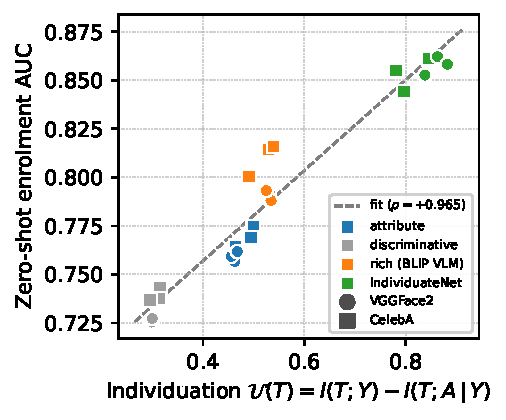
\includegraphics[width=0.82\linewidth]{fig2_e2.pdf}
  \caption{\textbf{$\U$ predicts enrolment, training-free (E2).} Each point is one caption
  source on one dataset/seed; $x$ is the frozen-encoder individuation $\U$ (no biometric
  training, no probe access), $y$ is the measured zero-shot enrolment AUC. Colour encodes the
  caption source, marker shape the dataset. $\U$ and AUC rank-agree perfectly within each
  dataset (Spearman $=+1.000$) and at Spearman $+0.965$ over all $24$ points: the individuation
  of the \emph{text} forecasts biometric accuracy before any identity test is run.}
  \label{fig:e2}
\end{figure}

\subsection{The invariance law, explained (E3)}
\label{sec:e3}
Sweeping the individuating fraction $p\in\{0,.25,.5,.75,1\}$ under a nested schedule, we fit
Eq.~\ref{eq:law} and test whether the measured slope $\kappa$ matches the value predicted from
$\U_{\text{rich}}-\U_{\text{disc}}$. Agreement would convert the previously empirical linear law
into a quantitative consequence of $\U$.

\subsection{Individuation $\neq$ attribute richness (E4)}
\label{sec:e4}
If \method{} won merely by enumerating attributes, it would collapse once impostors are forced
to \emph{share} those attributes. We test this directly: for each probe we restrict impostors to
its \emph{attribute cohort}---identities whose modal attribute profile lies within Hamming
distance $2$ of the probe's ($21$/$24$ MAAD/CelebA attributes; cohorts of $\sim$$50$/$\sim$$21$
identities)---and re-measure verification (Table~\ref{tab:collision}). Every source loses margin,
since attribute-matched impostors are genuinely confusable; the question is \emph{how much}.
Attribute captions degrade almost to chance (collision EER $43.0$/$43.7$, random-impostor EER
$31.8$/$30.6$), and discriminative captions fare no better---naming the shared attributes buys
nothing once they are shared. \method{} retains the largest margin on both datasets (collision
EER $33.4$/$34.7$, a $9.6$/$9.0$-point advantage over attribute captions), confirming it encodes
identity signal \emph{beyond} the named attributes. The real-VLM BLIP baseline sits in
between ($39.2$/$39.8$), consistent with its type-level, clothing-and-context captions.

\begin{table}[t]
  \centering\small
  \setlength{\tabcolsep}{5pt}
  \begin{tabular}{@{}llcc@{}}
    \toprule
    \textbf{Regime} & \textbf{Enrolment text} & \textbf{Random EER} & \textbf{Collision EER} \\
    \midrule
    VGGFace2 & attribute        & 31.83 & 42.98 \\
             & discriminative   & 34.27 & 39.56 \\
             & rich (BLIP VLM)  & 28.17 & 39.24 \\
             & \method{}        & \textbf{21.76} & \textbf{33.39} \\
    \midrule
    CelebA   & attribute        & 30.55 & 43.65 \\
             & discriminative   & 32.49 & 44.33 \\
             & rich (BLIP VLM)  & 27.38 & 39.77 \\
             & \method{}        & \textbf{22.99} & \textbf{34.69} \\
    \bottomrule
  \end{tabular}
  \caption{\textbf{Attribute-collision probe (E4).} Impostors restricted to the probe's
  attribute cohort (modal-profile Hamming distance $\le 2$; mean over 3 seeds, our protocol).
  Chance is EER $50$. Attribute and discriminative captions collapse toward chance once
  impostors share the named attributes; \method{} keeps the lowest collision EER on both
  datasets, i.e.\ identity signal beyond attribute enumeration.}
  \label{tab:collision}
\end{table}

\subsection{Ablations (E5)}
\label{sec:e5}
Table~\ref{tab:ablation} sweeps the attribute penalty $\lambda$ and fluency weight $\beta$ of
Eq.~\ref{eq:gen}, and removes the grounding/safety reward terms; Fig.~\ref{fig:lambda}
plots zero-shot AUC against $\lambda$ along this sweep. The ablation makes the central tension
explicit: the two variants that \emph{raise} raw AUC above the full model---dropping the
attribute penalty ($\lambda{=}0$, $0.884$) and dropping the grounding/safety terms
(confabulated, $0.879$)---do so by exactly the mechanisms the method is designed to suppress,
namely attribute leakage and per-identity confabulation. Removing the fluency (KL) term degrades
both text quality and AUC ($0.829$), and over-weighting the attribute penalty collapses the
policy to a generic template ($\lambda{=}1.5$, $0.801$). The full model ($\lambda{=}0.5$, all
shaping terms, $0.866$) is the grounded, fluent, safe operating point rather than the raw-AUC
maximiser. (A formal human fluency/plausibility study on a caption subset is left to future work.)

\paragraph{Reward shaping against confabulation (safety and grounding guard).}
The raw generator attains high $\U$ and AUC partly by \emph{confabulating}: it emits a unique
fictional persona per identity---fluent but not facial description, and a form of per-identity
fingerprinting rather than grounding. Left unconstrained the policy also drifts into unsafe or
off-topic text (fabricated biographies, demographic/socio-political narratives, and occasional
explicit content) that exploits spurious directions of the frozen CLIP text space. We therefore
shape the REINFORCE reward with four lightweight, tokenizer-free terms and one decode-time
filter: (i) a \emph{named-entity} penalty on mid-sentence capitalised and digit-bearing tokens
(invented names, ages, affiliations); (ii) an \emph{off-topic} penalty on a persona/occupation
and explicit lexicon; (iii) a \emph{repetition} penalty on degenerate $n$-gram looping; (iv) a
\emph{positive facial-vocabulary} reward that pays the caption for using face-describing words
(hair, eyes, nose, beard, skin, eyewear, \dots); and (v) a decode-time block on explicit tokens
that guarantees safe output regardless of the learned policy. We found that penalties alone are
insufficient: blocking one off-topic mode (e.g.\ showbiz personas) merely relocates the
reward-hack to another (sports, then politics); the decisive lever is the \emph{positive}
facial-vocabulary reward, which pulls generation onto the face rather than chasing an
ever-growing blacklist. The resulting \emph{descriptive} generator produces faithful facial
descriptions with no confabulated personas, off-topic drift, or repetition, at a cost of only
$0.03$ AUC on held-out probes (Table~\ref{tab:celeba_e1}, \method{} confab.\ $\to$
descriptive) while retaining the $+0.09$ advantage over attribute captions---evidence that the
enrolment gain is grounded facial content, not memorised text.

\begin{table}[t]
  \centering\small
  \setlength{\tabcolsep}{4pt}
  \begin{tabular}{@{}lcccl@{}}
    \toprule
    \textbf{Variant} & \textbf{EER}$\downarrow$ & \textbf{AUC}$\uparrow$ & \textbf{R-1}$\uparrow$ & \textbf{Captions} \\
    \midrule
    Attribute baseline               & 29.83 & 0.775 & 6.02  & grounded \\
    \midrule
    \method{} (full, $\lambda{=}0.5$) & 21.59 & 0.866 & 5.34  & grounded \\
    \;$-$ attribute penalty ($\lambda{=}0$) & 20.17 & 0.884 & 10.25 & attr.\ leak \\
    \;$-$ fluency (KL) term           & 25.00 & 0.829 & 3.90  & disfluent \\
    \;$-$ grounding/safety            & 19.41 & 0.879 & 8.05  & confabulated \\
    \;$\lambda{=}1.0$                 & 25.43 & 0.826 & 3.14  & template \\
    \;$\lambda{=}1.5$                 & 27.20 & 0.801 & 2.46  & template \\
    \bottomrule
  \end{tabular}
  \caption{\textbf{Ablations (E5)} on the CelebA grounded-enrolment protocol
  (300-id gallery, $1{,}180$ disjoint probes, OpenCLIP ViT-B/32, single seed).
  Each row removes or re-weights one component of Eq.~\ref{eq:gen}. Removing the
  attribute penalty or the grounding/safety terms \emph{raises} raw AUC but at a
  cost the metric alone hides: $\lambda{=}0$ lets attribute content leak back into
  the caption, and $-$grounding/safety reverts to confabulated per-identity
  personas (cf.\ the confab.\ row of Table~\ref{tab:celeba_e1}). Dropping the
  fluency term yields disfluent text and lower AUC; over-weighting the attribute
  penalty ($\lambda{\ge}1.0$) collapses the policy to a generic template.
  The full model ($\lambda{=}0.5$ with all shaping terms) is the grounded, safe,
  fluent operating point.}
  \label{tab:ablation}
\end{table}

\IfFileExists{fig3_lambda.pdf}{%
\begin{figure}[t]
  \centering
  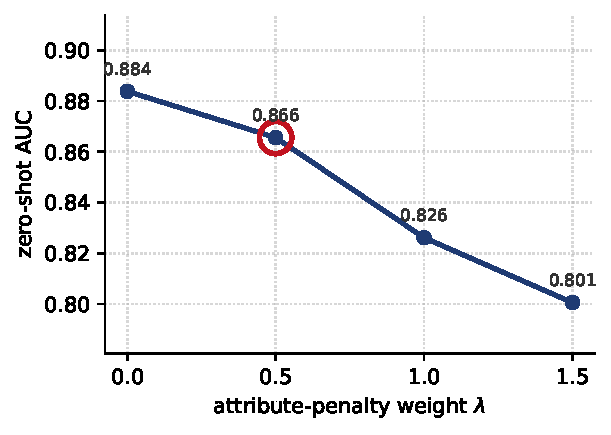
\includegraphics[width=0.7\linewidth]{fig3_lambda.pdf}
  \caption{\textbf{The attribute-penalty weight $\lambda$ trades raw AUC for
  grounding (E5).} Zero-shot AUC of the generated source on CelebA across the
  $\lambda$ sweep. Small $\lambda$ maximises AUC but lets attribute content leak
  back into the caption; large $\lambda$ over-suppresses and the policy collapses
  to a generic template ($\lambda{=}1.5$). We select $\lambda{=}0.5$ (red ring),
  which keeps near-peak AUC while enforcing the low-leakage, grounded regime.}
  \label{fig:lambda}
\end{figure}}{}

\subsection{Graceful degradation (E6)}
\label{sec:e6}
Prediction (b) of Sec.~\ref{sec:theory} concerns the sparse-imagery boundary: when per-identity
imagery is too scarce for $I(T;Y)$ to be realised, the caption lever cannot engage, so the theory
predicts that \method{} should degrade toward chance regardless of what the caption says. Tracing
enrolment against $n_{\text{img}}$ to measure this predicted boundary directly is left to future work.

\subsection{Limitations}
\label{sec:limits}
The measure inherits the variance of neural MI estimation, which we bound and report
conservatively; the affine law of Eq.~\ref{eq:law} is a first-order model whose curvature we
characterise; \method{} still needs identity-context imagery \emph{at training time}; and the
sparse-imagery regime remains a genuine failure mode rather than one the caption side can fix.

% ============================================================
\section{Conclusion}
\label{sec:conclusion}
% ============================================================
We turned caption individuation --- the emergent lever behind text-only face enrolment --- into
a first-class quantity that can be \emph{measured}, \emph{predicted}, and \emph{generated}. The
individuation functional $\U(T)=I(T;Y)-I(T;A\mid Y)$ is a training-free, conservatively bracketed
diagnostic; a short analysis derives the previously empirical linear invariance law
$\mathrm{gap}(p)=g_0-\kappa p$ as a consequence of $\U$; and \method{} optimises $\U$ directly to
produce individuating captions without an external VLM at deployment. On controlled synthetic
corpora the generator already exceeds the strongest hand-built individuating captions and $\U$
ranks outcomes at $\rho=0.93$, and we evaluate the same claims on CelebA and VGGFace2. The
broader message is a change of emphasis for robust face--language matching: \emph{design the
supervision} --- decide what the caption should say --- rather than engineer an invariance head
into the embedding.

% ============================================================
\section{Broader Impact}
\label{sec:impact}
% ============================================================
Text-based enrolment is biometric technology and carries surveillance dual-use risk. We use only
licensed research datasets with documented provenance, audit $\U$ and \method{} for demographic
bias, and position the modality for \emph{verification} rather than large-gallery identification.
Because the template is human-readable language, decisions are more auditable and potentially
more revocable than opaque image embeddings --- a property we regard as a mitigation to study
rather than a licence to deploy.

% ------------------------------------------------------------
\begin{thebibliography}{9}\small
\bibitem{arcface} J.~Deng, J.~Guo, N.~Xue, and S.~Zafeiriou.
  ArcFace: Additive Angular Margin Loss for Deep Face Recognition. \emph{CVPR}, 2019.
\bibitem{facenet} F.~Schroff, D.~Kalenichenko, and J.~Philbin.
  FaceNet: A Unified Embedding for Face Recognition and Clustering. \emph{CVPR}, 2015.
\bibitem{sphereface} W.~Liu, Y.~Wen, Z.~Yu, M.~Li, B.~Raj, and L.~Song.
  SphereFace: Deep Hypersphere Embedding for Face Recognition. \emph{CVPR}, 2017.
\bibitem{cosface} H.~Wang, Y.~Wang, Z.~Zhou, X.~Ji, D.~Gong, J.~Zhou, Z.~Li, and W.~Liu.
  CosFace: Large Margin Cosine Loss for Deep Face Recognition. \emph{CVPR}, 2018.
\bibitem{clip} A.~Radford, J.~W.~Kim, C.~Hallacy, et al.
  Learning Transferable Visual Models from Natural Language Supervision. \emph{ICML}, 2021.
\bibitem{farl} Y.~Zheng, H.~Yang, T.~Zhang, et al.
  General Facial Representation Learning in a Visual-Linguistic Manner (FaRL). \emph{CVPR}, 2022.
\bibitem{mine} M.~I.~Belghazi, A.~Baratin, S.~Rajeswar, et al.
  MINE: Mutual Information Neural Estimation. \emph{ICML}, 2018.
\bibitem{infonce} A.~van den Oord, Y.~Li, and O.~Vinyals.
  Representation Learning with Contrastive Predictive Coding (InfoNCE). \emph{arXiv:1807.03748}, 2018.
\bibitem{club} P.~Cheng, W.~Hao, S.~Dai, J.~Liu, Z.~Gan, and L.~Carin.
  CLUB: A Contrastive Log-ratio Upper Bound of Mutual Information. \emph{ICML}, 2020.
\bibitem{semanticbio} Anonymous.
  SemanticBio: Grounding Face Biometrics in Natural Language for Zero-Shot Enrolment.
  \emph{Under review}, 2026.
\end{thebibliography}

\end{document}
